\chapter{analysis}\label{analysis}

ToDo:
\begin{enumerate}[nosep]
    \item Datenformat Input, verwendete Daten, Worte zu Simulation, trainingsdaten
    \item Preprocessing - Schritte erklären
    \item Datenformat Output Preprocessing
    \item Signifikanzkurve
\end{enumerate}

\section{preprocessing}
% configuration in appendix! + algorithmen beim prep

\subsection{Monte Carlo Data (More Infos: number of events, \ldots)}
Our analysis is based on simulated monte carlo events
The particle shower simulation is done with the software CORSIKA, 
the simulation of the experiment goes by the name simtel.

Monte carlo (MC) data is simulated and shared across the CTA-collaboration, 
our analysis uses the data from the PROD3-simulation of 
the CTA-south array. These events have been simulated on
much larger arrays to simulate different layouts at once.
We will choose the relevant telescopes in a way, that
our array resembles the earlier mentioned south array (cite sec).

This data contains pretty much everything the telescopes are going to measure
plus MC information, that will not be present at real experiments.
This includes the simulated particle direction and energy.


At the lowest level our observed data consists of uncalibrated waveforms 
in the camera pixels.
We will perform all analysis steps that are needed for real data.
All relevant parameters are listed in the appendix.

To specify a specific event, we will identificate an event based on 
three layers:
\begin{enumerate}
    \item{Run-Id: This gives us non-event-specific information about the monte carlo run, e.g.
    spectral\_index, particle injection height, ...}
    \item{Array-event-id: Any shower that triggered the array is considered to be an array event.
    Array-level features consist of general event information 
    (e.g. number of triggered telescopes, average internsity)
    reconstructed features of the primary particle (energy, source position, ...) and the 
    event specific monte carlo information to compare these features against.}
    \item{Telescope-event-id: This specifies how a specific telescope has seen the shower and
    contains information about the telescope itself (e.g.focal length). Telescope-level features 
    describe the camera image, amongst other things via the hillas-parameters(cite stuff)}
\end{enumerate}
In the following we will 
distinguish between "array-events" and "telescope-events" when describing the reconstruction methods.

\subsection{Reconstruction on telescope level}
% definition datenlevel
- calibration
- cleaning
- hillas parameters 
- telescope level
- tabellen der features bei runs/arrays/telescopes

To be able to apply high-level analysis methods, the initial data 
needs to be reduced and preprocessed substantially.


Processing of the simtel-files is done with the aforementioned ctapipe, starting with 
the calibration of the event. This performs an integration of the waveforms in 
each pixel of the camera of a triggered telescope. Inside ctapipe the initial data is referred to as R1
and the resulting data as dl1. The resulting images get cleaned with a tailcuts approach
before they are
used to calculate image features, such as the hillas parameters.

Hier part über hillas params mit den bildern! erklären wieso und so

In addition to the original hillas parameters, the concentration, number of islands 
and timing parameters get calculated.
Concentration refers to the intensity captured in some subset of pixels relative to 
the total intensity in the image.
An island is considered a connected cluster of pixels. In an ideal gamma shower image, only one island
is expected, although this is highly dependend on the applied cleaning.
Timing parameters are the second momenta of the distribution of the relative peak arrival times
in each pixel, which can be derived form the waveforms.

All these features get used in the machine learning algorithms at later stages.

\subsection{Hillas reconstructor}  % we dont seperate between 0 and 1 right?
After the image processing of each associated telescope image has been finished,
the predictions of our "baseline" source position estimator get calculated.
This algorithm is referred to as HillasReconstructor inside ctapipe, because 
it works based on the hillas parametrisations of the images.
For each triggered telescope, a 2D-plane is drawn based on the main shower 
axis and the telescope orientation. These planes intersect and 
the weighted average of all intersections gives the 
direction of the shower origin,
see figure \ref{fig:hillas_reconstructor} (cite code or paper).

\begin{figure}
	\centering
	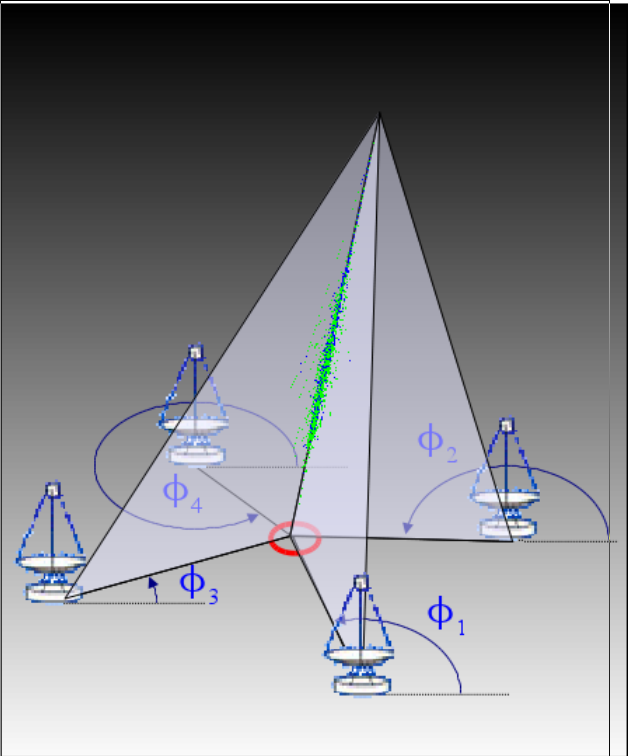
\includegraphics[width=0.8\textwidth]{images/hillas_reco.png}
	\caption{Hillas reconstructor}
	\label{fig:hillas_reconstructor}
\end{figure}

Since this method inherently requires a stereoscopic experiment
and multiple triggered telescopes, it will not work for a single telescope.
From earlier studies (kram zitieren, zb kai), it is expected
that this method works best with an event multiplicity 
(number of triggered telescopes) $\geq 3$ with higher multiplicity
leading to better results.

\section{Machine Learning, dl3?}
High level analysis of the preprocessed data is based on the use of
the aict-tools \cite{aict-tools} package which itself is based on
sklearn \cite{sklearn_api} for the machine learning algorithms.
The algorithm of choice is the Random Forest algorithm
as it is well suited for the use with tabluar data and tends to rarely overfit
(citation needed).
Model feature importance will be calculated
based on the sklearn functionality, which
uses a XXX algorithm.
Seperate models are trained for the tasks of signal/background
separation, signal energy estimation and signal source position
reconstruction.
The aict-tools have originally been developed for the FACT-experiment
(citation needed) which is a single IACT. For this reason
adaptions had to be made to perform a stereoscopic analysis.



\subsection{g/h sep}
For the task of gamma/hadron separation a random forest can be trained
using either only monoscopic information or also using array-level
information from earlier reconstruction steps.
Performance of the Classifier will be gauged based 
on the area under the curve.
Using stereoscopic information
generally improves the AUC by a few percent points.
The single telescope predictions can be combined by
simple functions such as the mean or median of the
single predictions to provide a prediction for the complete
array-event.
% features und kram


% \section{energy estimation}
% Energy estimation can be performed in the same way as the gamma/hadron
% separation. For this task there has been earlier work indicating
% the usefulness of a second machine learning model trained
% on the predictions of the first telesope-level model
% \cite{ba-lars}.

% I am thus going to present results based on either calculating the mean
% of the telescope level predictions and using a second random forest
% to improve the array level prediction.

\subsection{source position}
\label{sec:source_position}
The position on the shower axis can be estimated based on 
the hillas parameters and other image features, as 
explained in section \ref{??}
This method is known as the DISP-method in the
literature (citation needed). The general idea 
can be seen in figure \ref{fig:disp}.

\begin{figure}
    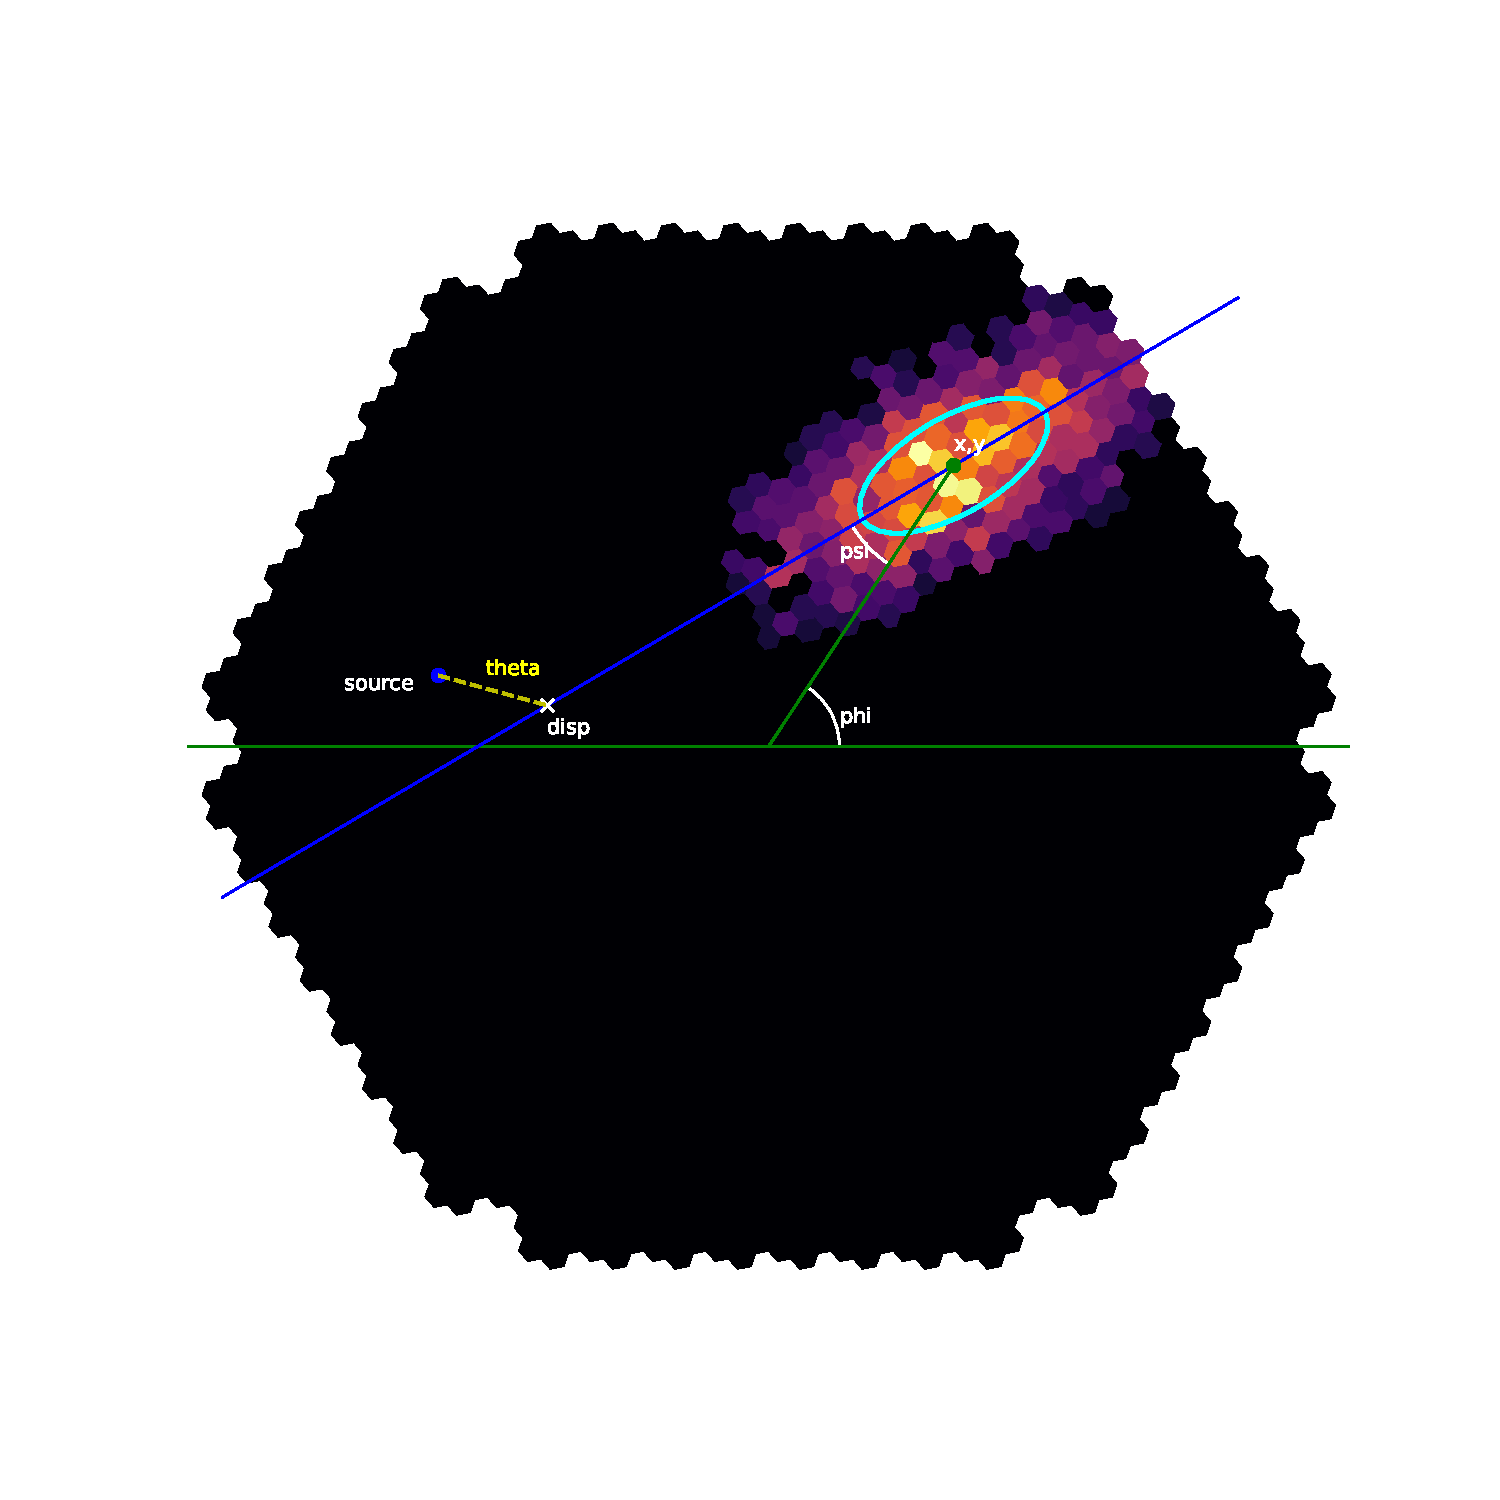
\includegraphics[width=0.6\linewidth]{Plots/hillas_complete.pdf}
    \caption{Illustration of monoscopic source position reconstruction making use of 
        the Hillas-Parameters and the DISP-method as explained in section \ref{sec:source_position}.
	A source position is estimated as some point on the main shower axis.
	In this example the head-/tail-ambiguation is guessed correctly.
	The position in the sky frame can then be calculated by transforming this
	point onto the sky plane.Pass das an zu 2 disps!}
    \label{fig:disp}
\end{figure}

With the DISP-method the estimated distance between the source
position and the center of gravity of the hillas ellipse gets calculated
based on the form of the ellipse, timing information and potentially
more features.
This will be done using machine learning models.
At this point the reconstructed source position
is fixed at two points at the main shower axis.

To resolve the head/tail ambiguity in monoskopic mode,
we will train a second random forest.
This is called SIGN-prediction, interpreting the two possible sides
as +-1, allowing for binary classification.
From FACT-analyses we know that accuracies of 70-80\% should be achievable
if we make no mistakes.

For the stereoskopic analysis, we employ an approach inspired by 
what the MAGIC-collaboration does in their analysis.
In the case of the MAGIC-telescopes the ambiguity does not
get resolved until the individual results get combined
on the stereo level. The choice of the correct
pair out of the four reconstructed positions can be done either
by calculating the crossing point of both main shower axises
or by calculating the pairwise distances between the positions \cite{magic disp paper}.


These methods are illustrated in figure \ref{fig:disp_magic}

\begin{figure}
    \begin{subfigure}{0.5\textwidth}
        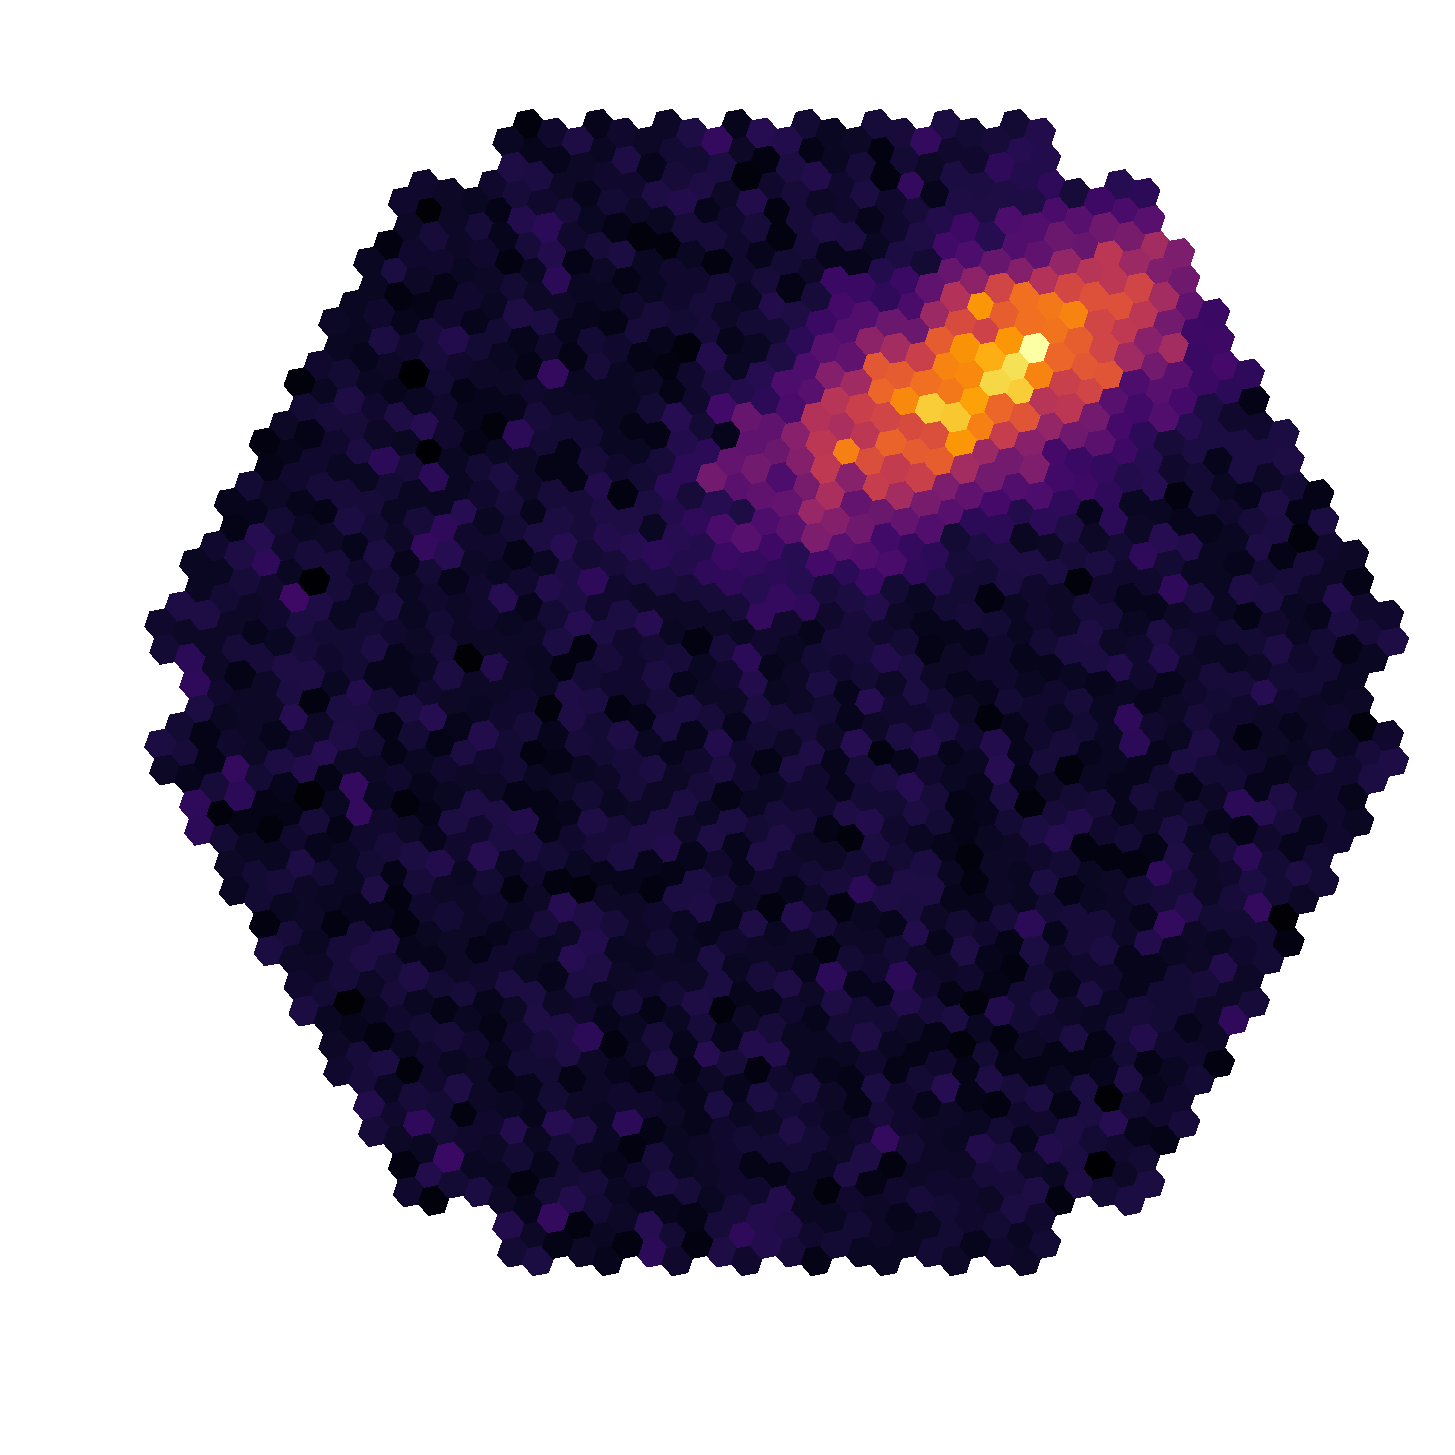
\includegraphics[width=0.9\linewidth]{Plots/hillas_raw.pdf} 
        %\caption{Caption1}
        \label{fig:3}
    \end{subfigure}
    \begin{subfigure}{0.5\textwidth}
        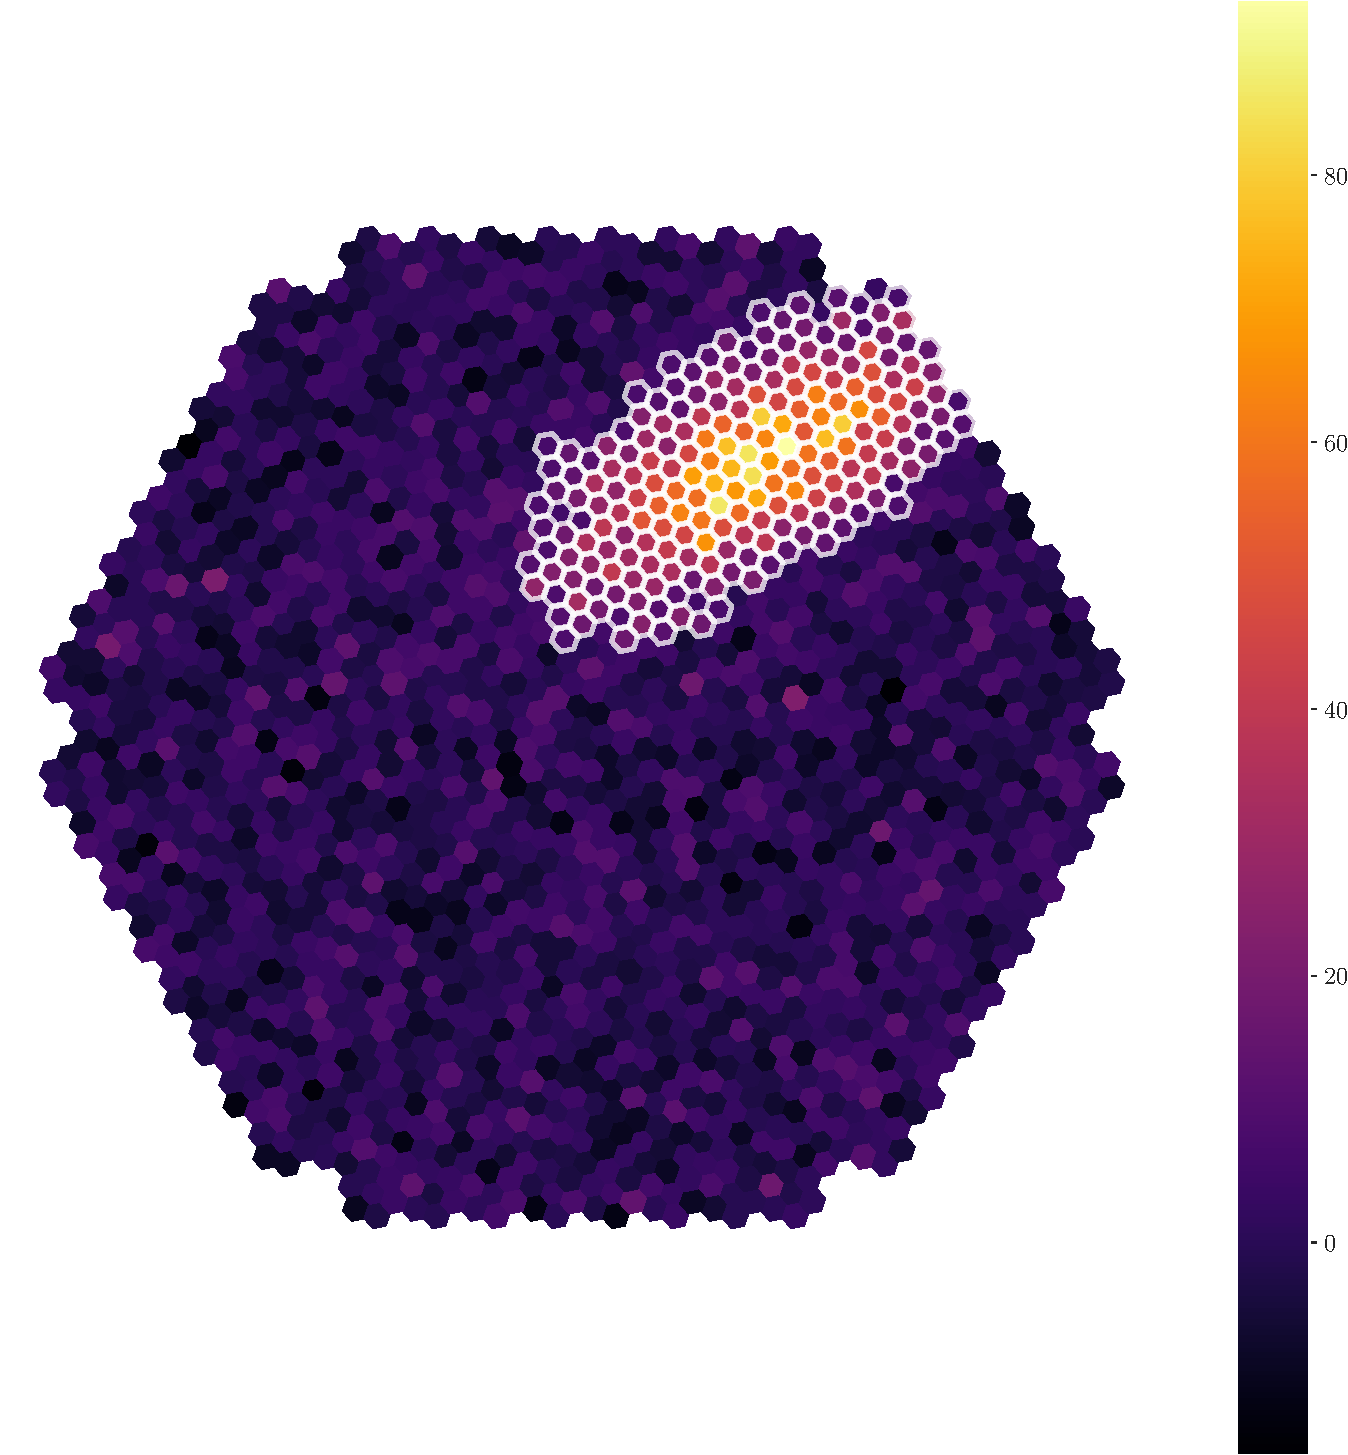
\includegraphics[width=0.9\linewidth]{Plots/hillas_cleaned.pdf}
        %\caption{Caption 2}
        \label{fig:2}
    \end{subfigure}
    \caption{wrong pics}
    \label{fig:disp_magic}
\end{figure}

Since we have a variable number of telescopes per (array) event,
we need to adapt this method in a scalable way.

The most obvious approach seemed to be an iterative one:
For each pair of triggered telescopes, we combine the results 
in the way described in \cite{disp magic paper}.
We cache all intermediate results and average them to get the final prediction.

Figure \ref{fig:stereo_disp} illustrates this for the case of 4 triggered telescopes.


\begin{figure}
    \begin{subfigure}{0.23\textwidth}
        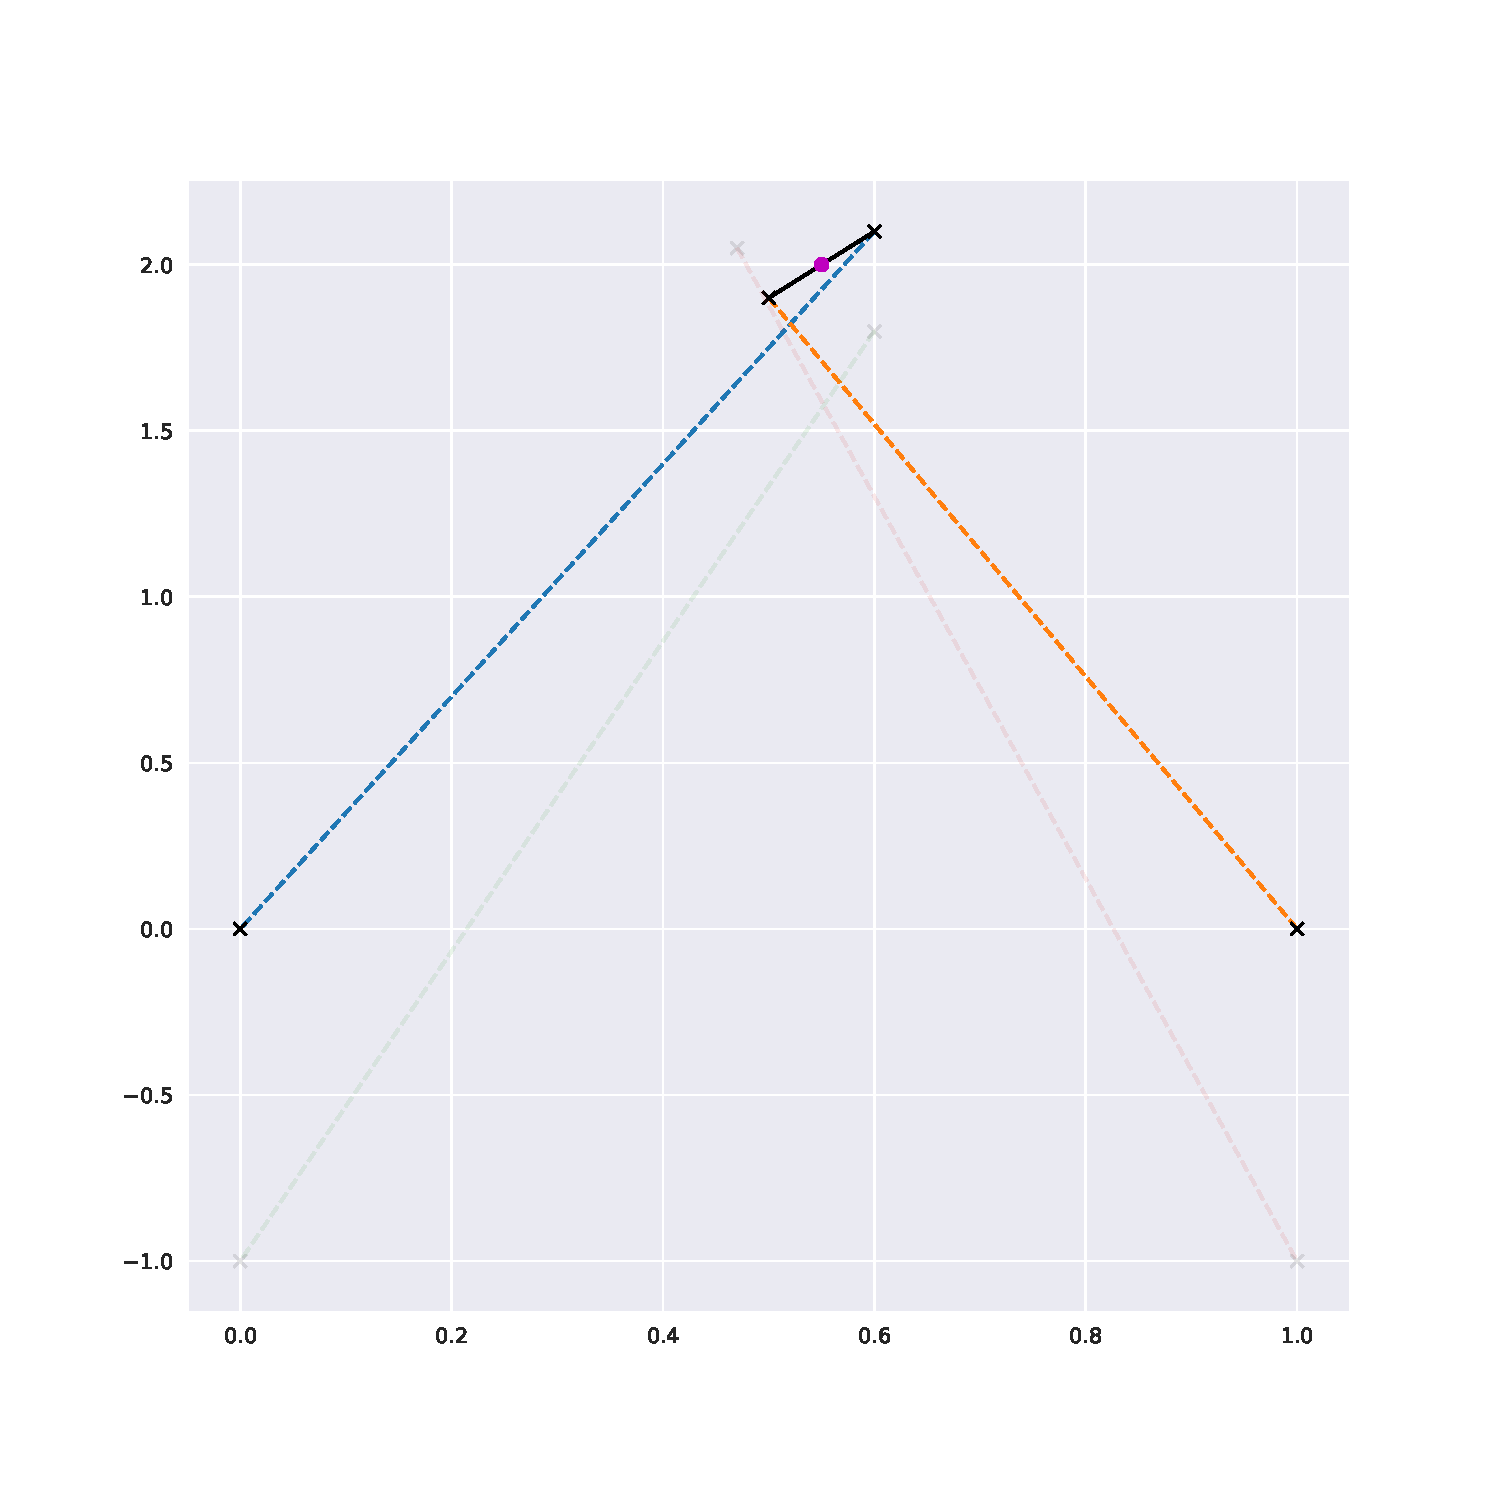
\includegraphics[width=0.9\linewidth]{Plots/stereo_magic_1.pdf} 
        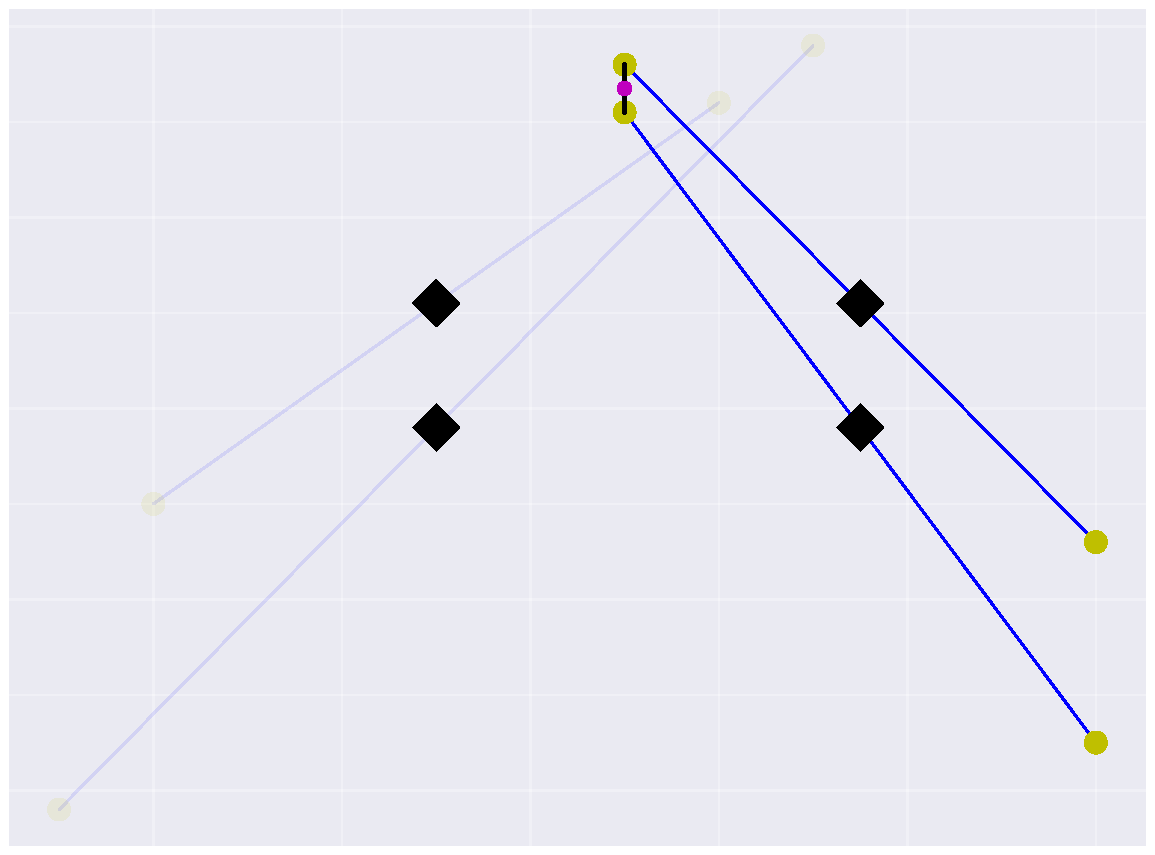
\includegraphics[width=0.9\linewidth]{Plots/stereo_magic_5.pdf} 
    \end{subfigure}
    \begin{subfigure}{0.23\textwidth}
        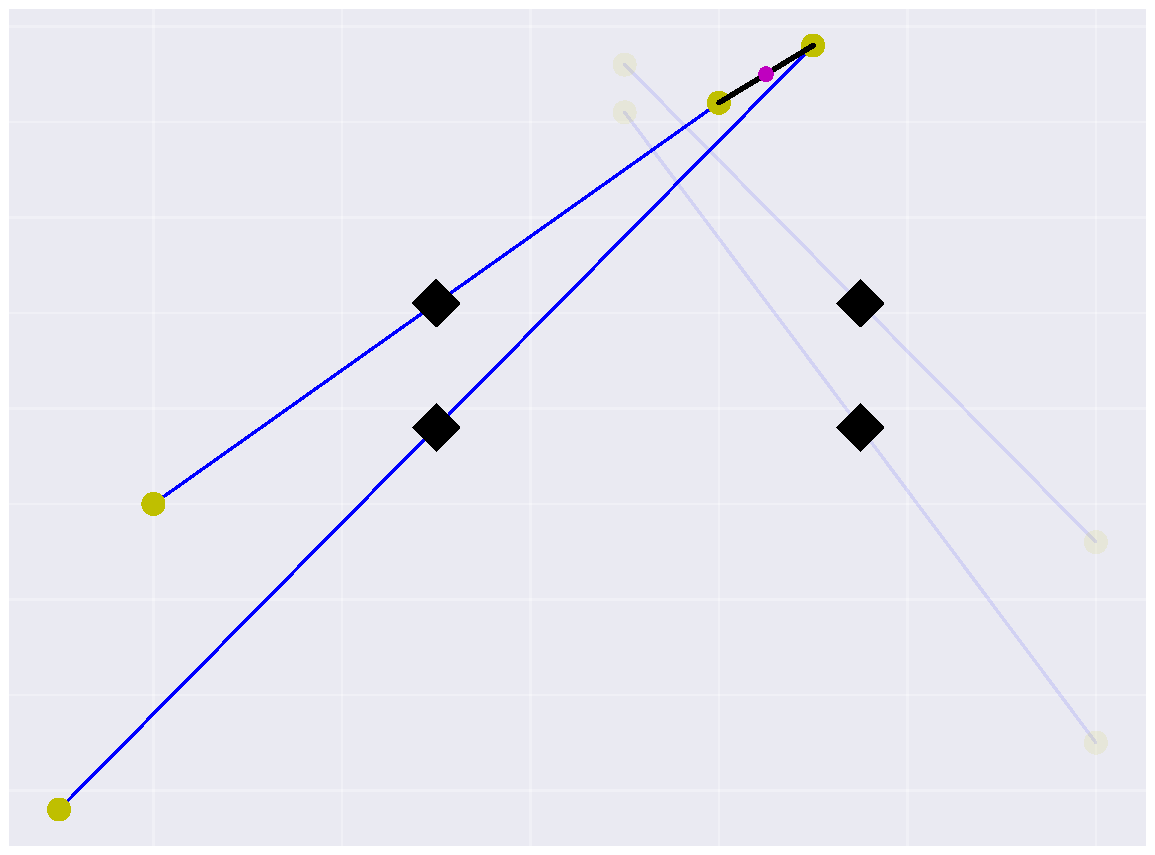
\includegraphics[width=0.9\linewidth]{Plots/stereo_magic_2.pdf}
        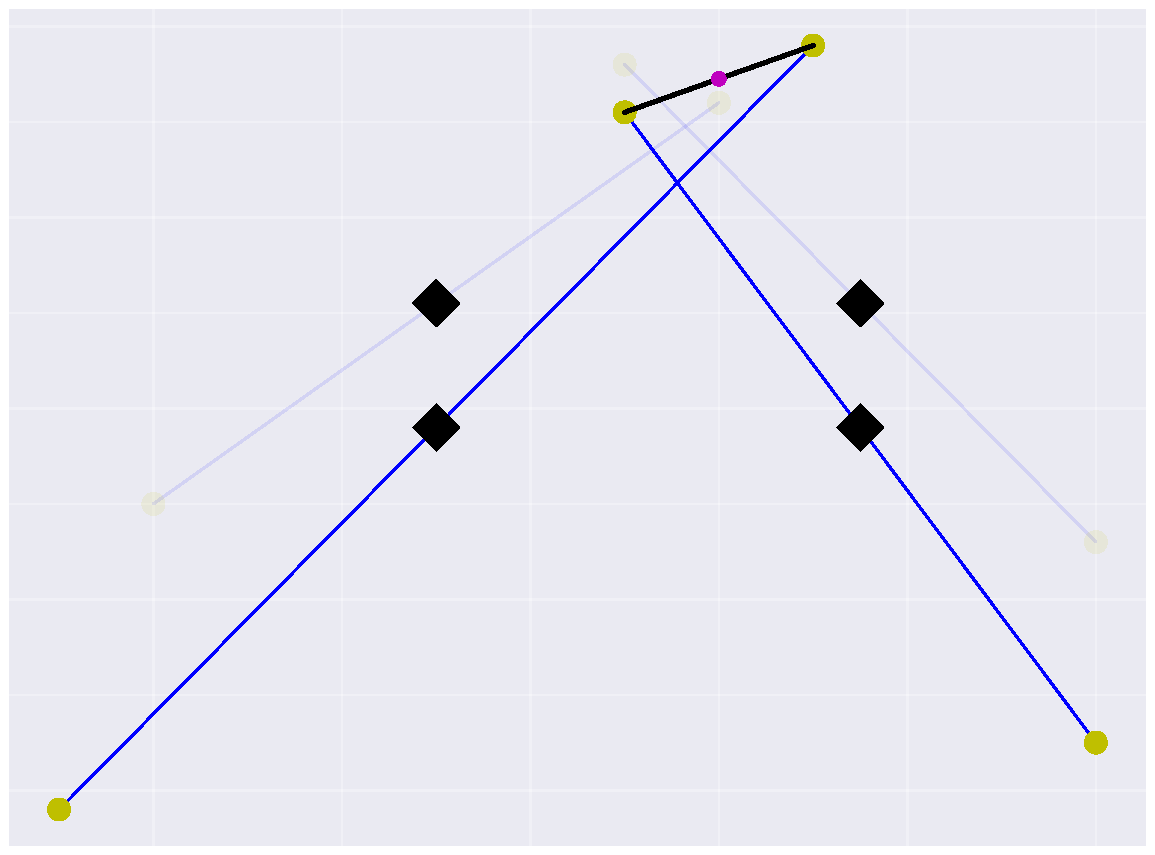
\includegraphics[width=0.9\linewidth]{Plots/stereo_magic_6.pdf}
    \end{subfigure}
    \begin{subfigure}{0.23\textwidth}
        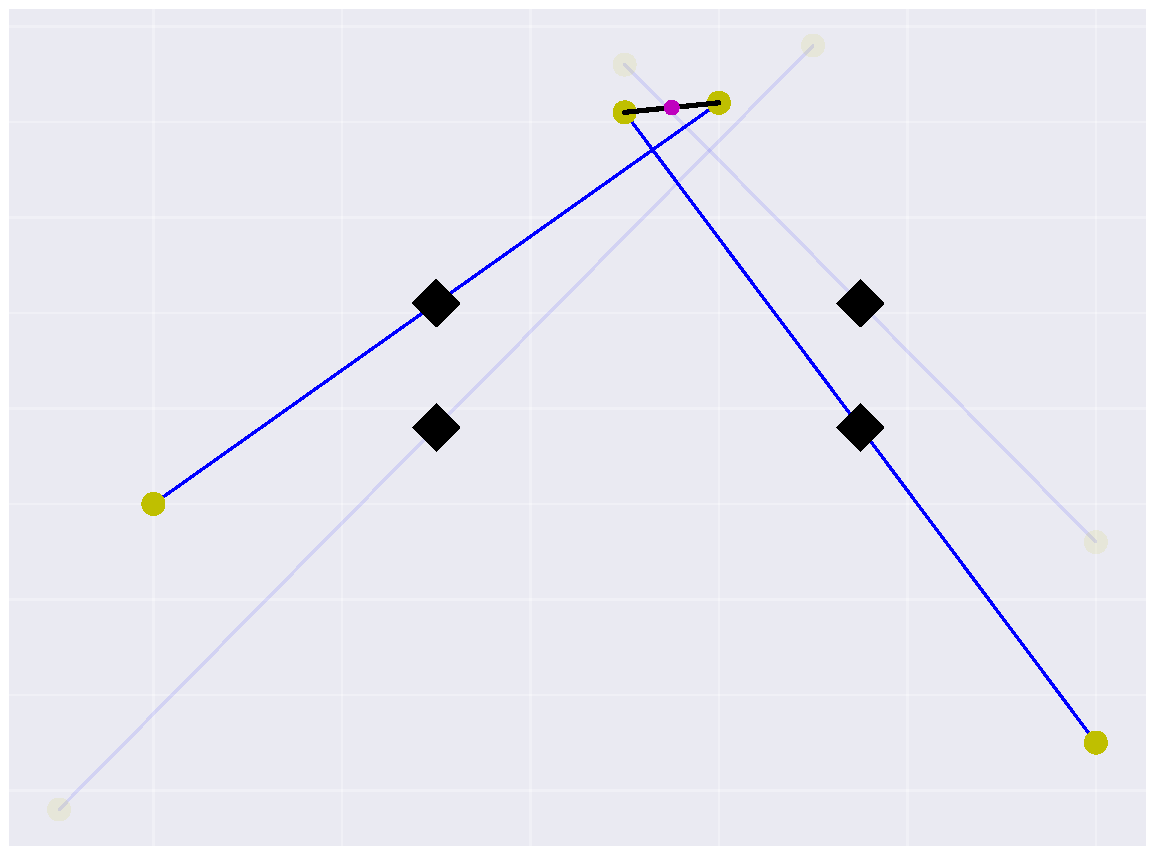
\includegraphics[width=0.9\linewidth]{Plots/stereo_magic_3.pdf} 
        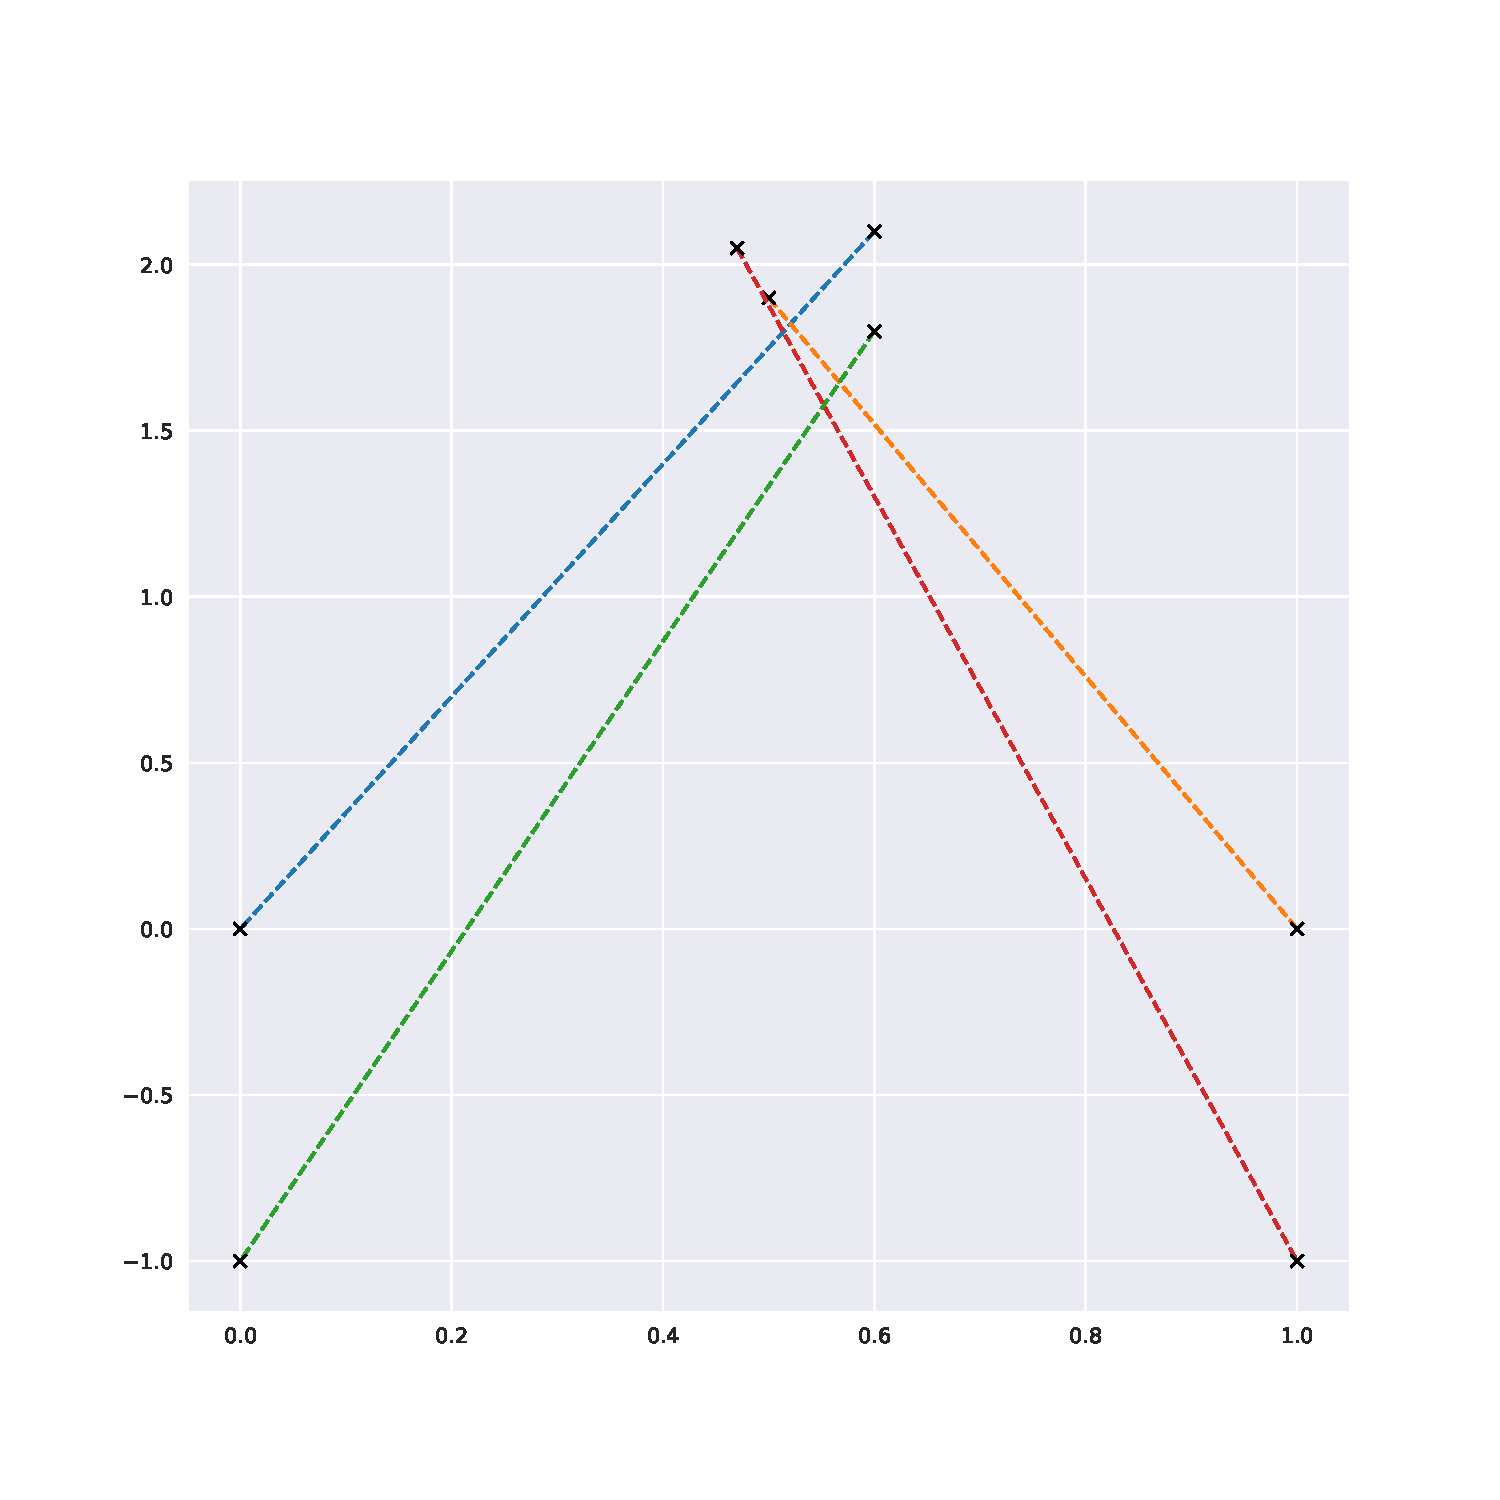
\includegraphics[width=0.9\linewidth]{Plots/stereo_magic_all.pdf} 
    \end{subfigure}
    \begin{subfigure}{0.23\textwidth}
        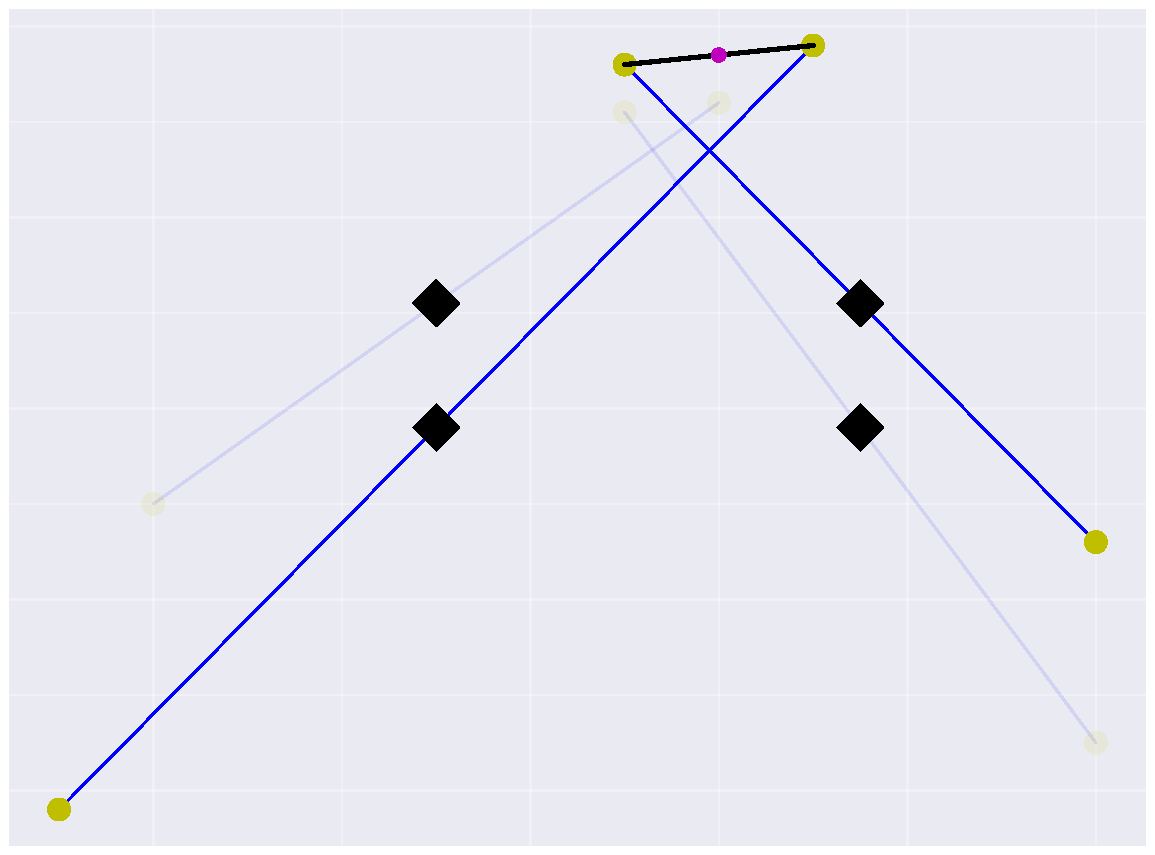
\includegraphics[width=0.9\linewidth]{Plots/stereo_magic_4.pdf}
        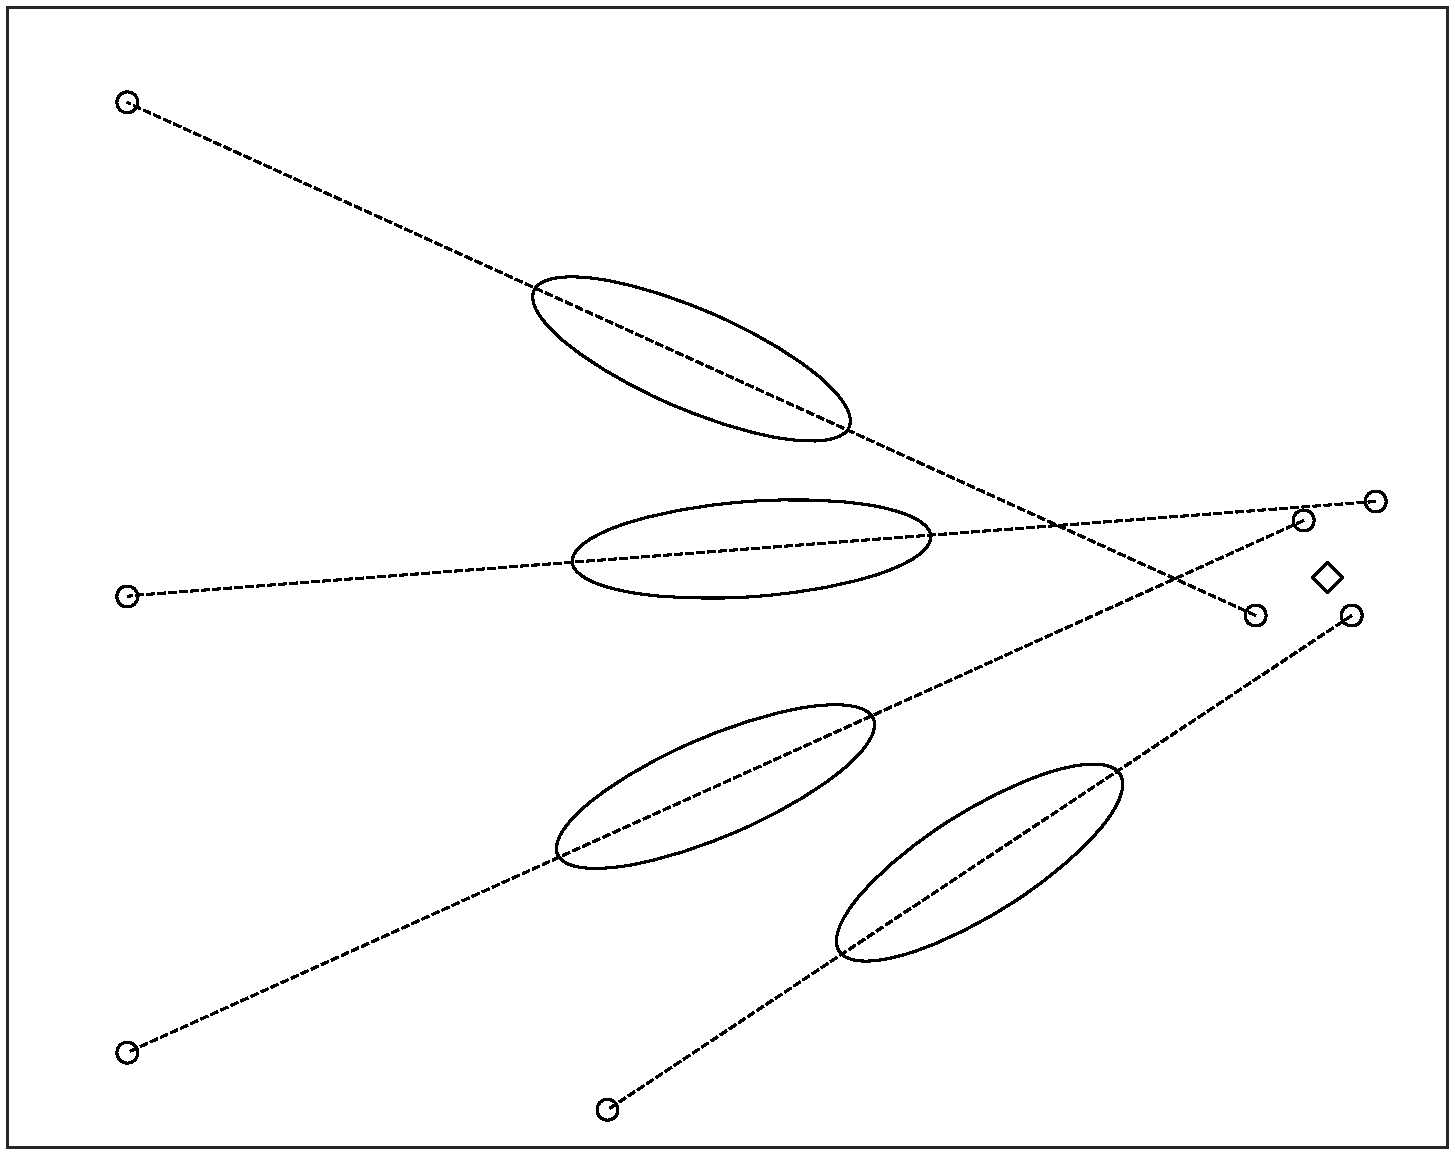
\includegraphics[width=0.9\linewidth]{Plots/stereo_magic_result.pdf}
    \end{subfigure}   \caption{wrong pics}
    \label{fig:stereo_disp}
\end{figure}


